\subsection{Framework Overview and Problem Formulation}
\label{sec:overall_framework}
\label{sec:problem_formulation}

HS-AeroTS is designed to connect runtime UAV telemetry anomalies with progressively more actionable diagnostic evidence. As illustrated in Figure~\ref{fig:hs_aerots_overview}, the framework follows three successive stages. First, multivariate PX4 telemetry is transformed into a window-level temporal-statistical representation and processed by a hierarchical predictor for anomaly detection and fault-domain diagnosis. Second, the diagnosed windows are interpreted using TreeSHAP, and feature-level contributions are aggregated into telemetry-channel, uORB-topic, and subsystem evidence. Finally, topic-level evidence is propagated through a firmware-specific PX4 uORB dependency graph to produce a ranked set of software modules for inspection.

\begin{figure}[htbp]
    \centering
    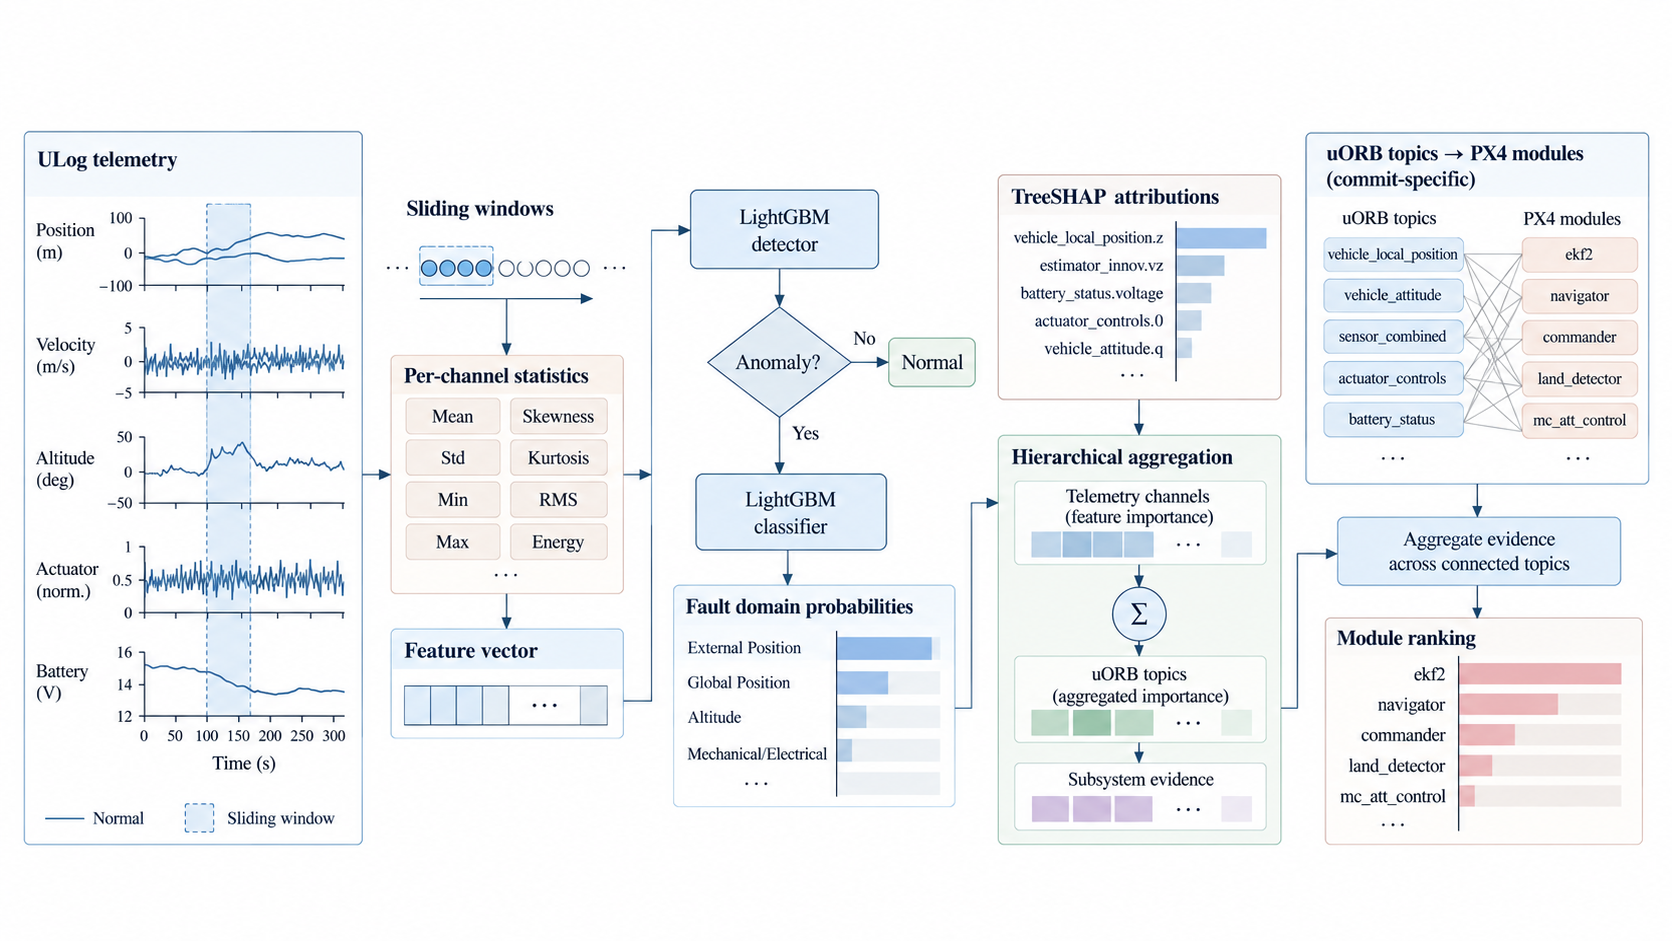
\includegraphics[width=\textwidth]{figures/figure_1_hs_aerots_overview.png}
    \caption{Overview of HS-AeroTS. Multivariate PX4 telemetry is transformed into temporal-statistical features for hierarchical anomaly detection and fault-domain diagnosis. TreeSHAP evidence is aggregated to engineering-level telemetry representations and propagated through a firmware-specific PX4 uORB graph to rank software modules for inspection.}
    \label{fig:hs_aerots_overview}
\end{figure}

Let the recorded-flight dataset be
\begin{equation}
\mathcal{D}
=
\left\{
\left(
\mathbf{X}^{(n)},
\mathcal{A}^{(n)},
v_n
\right)
\right\}_{n=1}^{N},
\label{eq:recorded_flight_dataset}
\end{equation}
where $\mathbf{X}^{(n)} \in \mathbb{R}^{T_n \times C}$ denotes the aligned multivariate telemetry of the $n$-th flight, $\mathcal{A}^{(n)}$ contains its available anomaly intervals and fault-domain annotations, and $v_n$ denotes the associated PX4 firmware revision. The flight duration $T_n$ may vary across logs, whereas $C$ denotes the retained telemetry channels.

Each flight is partitioned independently into temporal windows. For a window $w$,
\begin{equation}
\mathbf{x}_w \in \mathbb{R}^{L \times C}
\label{eq:telemetry_window}
\end{equation}
denotes its multivariate telemetry segment, which is transformed into a temporal-statistical representation
\begin{equation}
\mathbf{f}_w = g(\mathbf{x}_w) \in \mathbb{R}^{D},
\label{eq:temporal_statistical_representation}
\end{equation}
where $g(\cdot)$ denotes the telemetry representation function and $D$ is the resulting feature dimension.

The diagnostic task is organized hierarchically. The first stage estimates the probability that a telemetry window is anomalous,
\begin{equation}
p^{a}_{w}=h_{1}(\mathbf{f}_{w}),
\label{eq:anomaly_probability}
\end{equation}
where $p^{a}_{w}\in[0,1]$. A window is forwarded to fault-domain diagnosis when $p^{a}_{w}$ exceeds an operating threshold $\tau$. For a detected anomalous window, the second stage predicts a probability distribution over four annotated fault domains,
\begin{equation}
\mathbf{p}^{d}_{w}=h_{2}(\mathbf{f}_{w}),
\label{eq:fault_domain_probability}
\end{equation}
with
\begin{equation}
\mathcal{Y}_{d}
=
\{
\text{External Position},
\text{Global Position},
\text{Altitude},
\text{Mechanical/Electrical}
\}.
\label{eq:fault_domain_label_space}
\end{equation}

The resulting hierarchical prediction is
\begin{equation}
\hat{y}_{w}
=
\begin{cases}
\text{Normal}, & p^{a}_{w} \leq \tau,\\[4pt]
\displaystyle \arg\max_{k\in\mathcal{Y}_{d}} p^{d}_{w,k},
& p^{a}_{w} > \tau.
\end{cases}
\label{eq:problem_cascade}
\end{equation}

For each diagnosed anomalous window, HS-AeroTS further derives class-specific diagnostic evidence from the prediction model and converts it into an architecture-aware ranking over PX4 software modules. The overall objective is therefore not only to determine whether abnormal behavior occurs, but also to associate a detected anomaly with a fault domain and a traceable set of telemetry and software inspection candidates.
